\documentclass[a4paper,10pt]{article}

\usepackage{ifpdf}
\ifpdf
  \usepackage[pdftex]{graphicx}
  \graphicspath{{images/}}
\else
  \RequirePackage[dvipdfm, CJKbookmarks, bookmarks=true, bookmarksnumbered=true%
                unicode,%
             colorlinks,%
         citecolor=blue,%
             hyperindex,%
       plainpages=false,%
      pdfstartview=FitH]{hyperref}
  \AtBeginDvi{\special{pdf:tounicode UTF8-UCS2}}
  \usepackage[dvipdfm]{graphicx}
  \graphicspath{{images/}}
  \DeclareGraphicsExtensions{.eps}
\fi

%\RequirePackage{CJKutf8,CJKnumb,CJKulem}
\RequirePackage{CJKutf8,CJKnumb}
\RequirePackage{color,verbatim,cite}
\RequirePackage{texnames,makeidx,indentfirst}
\RequirePackage{amsmath,amssymb,amsfonts,bm,manfnt}
\RequirePackage{fancyhdr,titlesec,datetime}
\RequirePackage{wasysym,longtable,multirow,bigstrut}
\usepackage[section]{placeins}
\usepackage[left=2.54cm,right=2.54cm,top=3.3cm,bottom=2.6cm]{geometry}
\usepackage[caption=false,font=footnotesize]{subfig}

\AtBeginDocument{\begin{CJK*}{UTF8}{song}\CJKtilde\CJKindent\CJKcaption{utf8}}
\AtEndDocument{\end{CJK*}}

\setlength{\parskip}{0.75ex plus .2ex minus .5ex}
\renewcommand{\baselinestretch}{1.2}

\hypersetup {
    pdftitle={无线传感器网络中的位置相关安全},
    pdfauthor={杨文博}
}

\title{无线传感器网络中的位置相关安全}
\author{杨文博}

\begin{document}

\maketitle

\section{项目的立项依据} 

(研究意义、国内外研究现状及发展动态分析,需结合科学研究发展趋势来论述科学意义;或结合国民经济和社会发展中迫切需要解决的关键科技问题来论述其应用前景。附主要参考文献目录)

上世纪末到本世纪初,通信、嵌入式和分布式计算技术有了飞速的发展,同时得益于微机电系统的长足进步,人们研制出各种不同功用的廉价微型传感器。这些传感器可以感知、测量并收集所处的环境信息,经过通信网络传输给传感器的部署者。无线传感器网络就是由大量支持无线通信的廉价传感器节点组成的分布式、自组织的无线网络。它可以广泛使用在国防军事、国家安全、环境检测、火灾预警、仓储物流、交通管理、医疗卫生和灾难救援等许多领域,帮助人们及时获得有价值的目标环境信息,协助管理者做出正确的决策。\cite{Capkun2006a}

无线传感器节点一般情况下由感应模块、处理器、内存、能量供应、无线模块和控制单元组成。装配着不同的感应模块的传感器可以感知和测量物理环境的不同信息,例如湿度、温度、压力、震动、风速、声音、辐射、有毒气体含量等等,因而可以应用于不同的环境中。由于其廉价性和微型化,无线传感器所采用的处理器一般比较低端,不支持如浮点运算、多媒体指令等一些高级功能。它们一般都只配备少量的内存,所收集到的信息将使用无线方式传输到基站。一般情况下,无线传感器节点的能量主要由电池供应,根据环境的不同可以采用太阳能等其它的能量供应方式作为后备能源。

典型的无线传感器网络一般由数十到数千个无线传感器节点组成,由人工或者机械撒播在目标区域,用来监测目标区域内的特定环境信息。受无线传感器节点体积小、数量大、资源受限的限制,无线传感器网络往往具有以下特点:

\begin{enumerate}

\item 通信的带宽、稳定性和安全性较差。由于采用无线信号通信,受信道本身物理特性的限制,无线传感器网络的通信质量和稳定性往往较差;考虑到无线信号的开放性,其更容易受到信道窃听、伪装、拒绝服务等攻击,需要考虑一些特别安全需求。

\item 网络资源受限。无线传感器节点往往不具有长期的电源供应,节点设计的计算能力、存储空间都要比一般的有线网络节点要小得多。在设计网络网络结构时需要特别考虑到能耗因素,避免部分节点能源耗尽导致整个网络失灵。

\item 树形路由、多跳转发。基站是收集信息的汇聚点,所以无线传感器网络一般构成以基站为根节点的树形结构;由于节点天线发射功率小,信号的覆盖范围受限,无线传感器节点间通信往往需要经过多跳转发,其转发由传感器节点完成,没有专门的路由设备。

\end{enumerate}

由于受到上述特点的限制,无线传感器网络的组网、路由、数据传输的稳定性和安全性在设计时都需要特别考虑。

虽然面临着许多困难,但是由于其广泛的应用前景,无线传感器网络在工业应用和技术研发方面保持着非常强劲的增长势头。专注于无线技术的市场调研公司~ON World~在~2007~年~9~月发布的报告《无线传感器网络产业》中预计到~2011~年,世界市场无线传感器网络系统与服务价值将升至约~46亿~美元,比~07~年增长~5~亿美元~\footnote{ON World Research: \href{http://onworld.com/smartindustries/}{WSN for Smart Industries - A Market Dynamics Report }};市场研究机构~WTRS (West Technology
Research Solutions)~在~2008~年~12~月发布的《无线传感器网络技术趋势报告》中预测可用于无线传感器网络的低功耗~WiFi~芯片市场将在~2008~到~2013~年间保持~322\%~的复合年均增长率~\footnote{WTRS: \href{http://www.wtrs.net/wcntechtrends.htm}{Wireless Sensor Network Technology Trends Q4 2008}};ON World~公司~2009~年~1~月发布的《无线传感器网络研发趋势》报告预测到~2012~年,全球无线传感器网络研发支出将达到~13~亿美元,是~2007~年研发支出的~2.5~倍~\footnote{ON World Research: \href{http://onworld.com/wsn/}{Wireless Sensor Networks — R\&D Trends and Funding Opportunities }}。

我们可以看到,对无线传感器网络的研究,不仅是科技发展战略上的需求,而且在工业应用和服务上也有非常广大的发展前途。由于无线传感器网络往往用于监控敏感信息,或者部署在危险或者充满敌意的环境中,无线传感器网络的安全通常会受到严重的威胁。因此对其安全技术的研究是无线传感器网络研究中非常重要的一环,没有保证网络安全的技术,就不可能有可用的无线传感器网络。

位置信息是无线传感器网络中的一项重要信息。比如在环境监测的应用中,监测程序根据传感器所收集到的环境信息,检测是否有事件发生。在某事件发生时,管理者往往需要知道该事件发生的位置以及感知该事件的传感器节点的位置。没有位置信息的事件报告是不完整的,也是没有用处的。无线传感器节点的位置信息有着非常广泛的应用,包括数据的识别和关联、节点定位、对指定区域节点的管理和查询、评估节点密度和覆盖范围、网络能量分布图、基于地理位置的路由、目标追踪等。因此,保证节点正确、安全地获得和使用位置信息,对无线传感器网络的应用有着非常重要的作用。

虽然对无线传感器网络定位技术的研究起步较早,但无线传感器网络安全定位技术却是一个相对较新的研究课题,对其系统的研究起源于~2003~年左右。目前来讲,无线传感器网络的安全定位技术按照其算法和实现方式可以大致分为用密码学手段、异常行为检测和屏蔽、攻击容忍的鲁棒位置算法和位置验证技术等几大类~\cite{Boukerche2008},如图~\ref{wsn_sec_pos}~所示。下面我们对这几大类技术进行一些简单的说明和分析。

\begin{figure}[htbp]
  \centering
  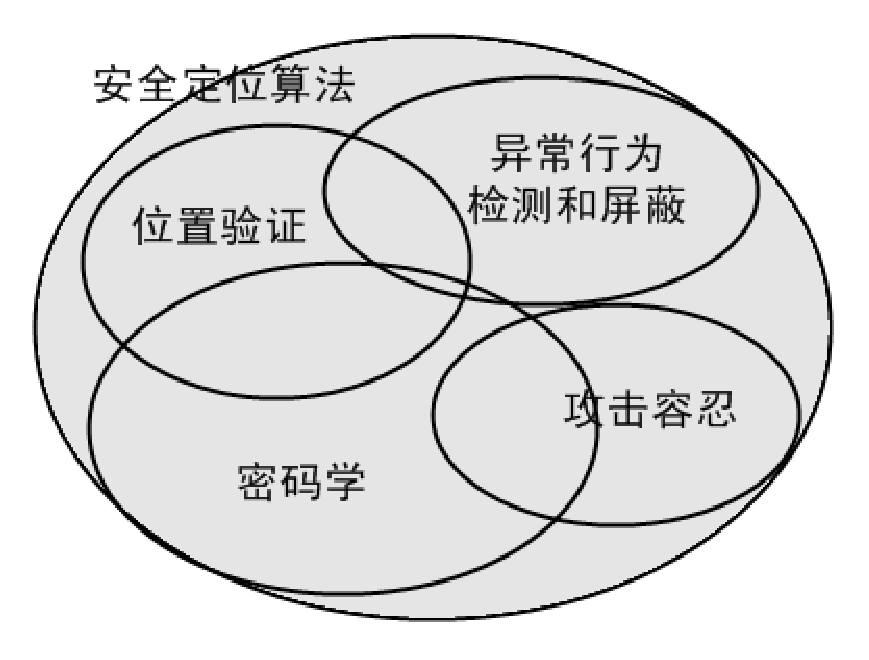
\includegraphics[width=.9\textwidth,keepaspectratio]{wsn_sec_pos}
  \caption{\label{wsn_sec_pos}~WSN~安全定位算法}
\end{figure}

\begin{itemize}

\item 密码学手段(Security through Cryptography)。密码学是保证信息安全的重要工具之一,因此也被广泛用于保护定位系统传输数据的安全中。数据包加密和数据源认证是安全定位系统中被广泛采用的密码学手段。

L. Lazos~和~R. Proovendran~等人提出的~SeRLoc \cite{Lazos2005}、~ROPE \cite{Lazos2006}~和~HiRLoc \cite{Lazos2005a},S. \v{C}apkun~和~J.P. Hubaux~提出的~SPINE \cite{Capkun2005, Capkun2006}~等方案,都采用了加密和数据源认证方法来保证~beacon~消息的安全传输。其中~SeRLoc~主要依靠已知自身位置的定位者节点,利用定向天线向扇形区域广播包含其自身位置和扇区信息的~beacon~信号,其它节点通过接收到的~beacon~信号判断自己处于哪些扇区内,这些扇区相交区域的重心就是该节点的位置。SeRLoc~采用全局的密钥来加密~beacon~消息,用私密口令的~hash~值链实现对~beacon~的消息源认证~\cite{Lazos2005}~(range-independent);SPINE~中提出了可验证的多向法(Verifiable Multilateration),第一次将距离边界协议(Distance Bounding Protocol)引入~WSN~位置验证中,在~VM~中至少三个验证节点独立使用距离边界协议计算某节点的位置,并将计算得的距离上传到一个~CA(Central Authority)~,CA~使用最小均方误差(Minimum Mean Square Error, MMSE)或者其它方法来估计得该节点的位置,并验证其是否在误差范围和扇区相交区域内,如果是就承认该距离估计有效。在~SPINE~方案中,距离边界协议使用了加密的挑战应答过程,需要节点与定位者共享对偶密钥~\cite{Capkun2005}~(range-based);ROPE~方案在~SeRLoc~基础上增加了距离边界协议,节点和能与其双向通信的定位者节点计算可信距离,配合扇区相交区域计算出节点位置。节点同样可以使用距离边界协议向某定位者节点证明自己在某位置附近,但是~ROPE~的过程不需要~CA~的参与。ROPE~同样要求所有节点与所有定位者共享对偶密钥~\cite{Lazos2006};HiLoc~是在~SeRLoc~的基础上,利用可旋转和可变发射功率的定向天线来达到高精度定位的目的。它与~SeRLoc~相同,也使用全局的密钥来加密~beacon~消息,用私密口令的~hash~值链实现对~beacon~的消息源认证~\cite{Lazos2005a}。

\item 异常行为检测和屏蔽(Misbehavior Detection and Block)。防范对定位系统的攻击还可以使用检测恶意节点的异常行为并屏蔽该恶意节点的方法。此方法主要用来防范对定位算法中位置计算部分的攻击。D. Liu~等在~\cite{Liu2005c}~提出了两个检测恶意~beacon~节点的方法:一个是节点用其与目标节点的坐标距离和实测距离(由信号估计得来)相比较,如果误差大于某个阈值,就认为该目标节点传输了虚假的坐标值,视其为恶意节点;另一个是节点用其与目标节点的通信往返时间与正常往返时间比较,如果误差大于某个阈值,则认为该目标节点进行了重放攻击,视其为恶意节点。A. Srinivasan~等在~\cite{Srinivasan2006}~中提出了一个分布式的基于信誉的~becon~信任系统(Distributed Reputation-based Beacon Trust System, DRBTS)。每个~beacon~节点维护一个邻居~beacon~节点的信誉表(Neighbor-Reputation-Table, NRT),节点间交换~NRT~,使用基于投票的方式选择可信节点组。

\item 攻击容忍的鲁棒位置算法(Robust Position Computation)。解决恶意节点问题的另一种办法是接受恶意节点存在这一现实,使用鲁棒的位置计算方法来消除恶意信息的影响。研究者一般假设正常节点多于恶意节点,然后使用统计或者异常值过滤(outlier filtering)技术来实现消除恶意节点影响的目标。这些方法一般用来防范对定位算法中位置计算或者位置/角度估计部分的攻击。

D. Liu~等在~\cite{Liu2005b}~中提出了攻击容忍的两个方案:第一个方案利用最小均方误差估计(Minimum Mean Square Estimation, MMSE)来识别并排除恶意节点。节点首先用基于~MMSE~的方案估计自身位置,然后看该位置能否由一个一致的参考者节点集合推出(距离估计的均方误差作为非一致性的参数),如果均方误差比较大,那么就剔除参考点集合中最不一致的节点重新估计位置,直到所有非一致节点都被剔除;第二个方案基于投票机制。WSN~部署区域被量化成网格,每个参考者节点对某节点所在位置进行投票,得票数最多的网格区域中央被选为该节点所在位置,这样能降低恶意节点在网络中的作用。D. Liu~等在~\cite{Liu2008a}~中又改进了~\cite{Liu2005b}~中提出的方案,提出一个增强的贪心~MMSE~算法(Enhanced Greedy Algorithm, EARMMSE),使用贪心算法减少了恶意节点识别和排除过程的计算量。

L. Fang, W. Du~和~P. Ning~在~\cite{Fang2005}~中提出了一个不需要~beacon~节点的位置计算方案~KPS(deployment Knowledge-based Positioning System),在~KPS~中节点根据预知的部署信息和当前的邻居节点,使用最大似然估计(Maximum Likelihood Estimation, MLE)方法计算自身可能的位置。该方案可以容忍小部分邻居节点是恶意节点的情况。

Z. Li~等在~\cite{Li2005a}~中提出了使用自适应的最小二乘法(Least Squares, LS)和最小均方算法(Least Mean Squares, LMS)的统计方法来容忍对定位算法的攻击。具体做法是在使用三角方法(Triangulation)估计节点位置时,无攻击存在时使用~LS~算法,当有攻击存在时使用~LMS~算法,因为~LMS~算法能够容忍不超过~50\%~的异常值并且获得正确估计。

\item 位置验证技术(Location Verification)。位置验证也是安全定位研究中非常重要的一个方面,它将视角从直接解决安全定位问题转向验证定位结果是否正确。我们前文中提到的一些方案,比如~SPINE \cite{Lazos2005a}, ROPE \cite{Lazos2006}~和~HiLoc \cite{Lazos2005a}~,也在安全位置计算过程中加入了位置验证过程。

N. Sastry~等在~\cite{Sastry2003}~中首先提出安全位置验证(Secure Location Verification)的概念,并给出了一个~Echo~方案,主要原理是使用无线射频和超声波测距的距离边界协议。原始~Echo~方案中使用~nonce~来抵御重放攻击,~\cite{Sastry2003}~中也提到在存在共享密钥的情况下,可以使用共享密钥来对消息源进行认证。

W. Du, L. Fang~和~N. Peng~基于~KPS~\cite{Fang2005},提出了一个在定位过程结束后,检测位置异常的节点~LAD(Localization Anomaly Detection)~\cite{Du2006}~方案。此方案中,节点被分组部署,根据部署信息和定位结果,若某节点的声称位置与其所属组节点的位置差距过大,则认为该节点位置异常。

S. \v{C}apkun, M. \v{C}agalj~和~M. Srivastava~提出了利用可信的隐藏和移动基站来对节点的位置进行验证的方案~\cite{Capkun2006a, Capkun2008}。由于部分基站位置隐藏(无线电静默)或者移动,攻击者无法判断该类基站位置,该类基站通过监听信道可以获得更真实的数据,判断节点是否处于声称的位置。

\end{itemize}

目前保护~WSN~节点位置信息私密性的研究并不多。~M. Gruteser~等在~\cite{Gruteser2003}~中首先提出使用数据隐藏(降低数据精度)、分层数据融合和加密通信的方法保证位置信息的私密性;C. Ozturk, Y. Zhang~和~W. Trappe~提出了利用抵抗流量分析的手段来防止敌手通过追踪通信得到节点位置,主要使用随机路由和增加虚假流量的方式~\cite{Ozturk2004},这些方式的主要问题是为了达到匿名性引入不必要的通信,因而使得能量消耗过大~\cite{Xiao2006};Y. Xi~等对~C. Ozturk~的方法进行了改进,提出了使用双向贪心随机游走的~GROW(Greedy Random Walk)~方案~\cite{Xi2006},~GROW~要求消息的发送者和接收者都进行若干跳的随机游走,当发送者和接收者的随机游走路径发生交叉时,就用该路径进行消息的传输。

~WSN~节点的位置信息在其它安全服务中也有一定的应用。D. Liu~和~Peng Ning~认为可以利用~WSN~节点的部署信息来减少密钥预分配的复杂度,提出了两个方案:CPKS(Closest Pairwise Keys Scheme)~和~LBKP(Location-Based Key Predistribution)\cite{Liu2003}。前者利用准确的周围临近节点信息预分配对偶密钥,后者将部署区域划分成块,使用基于二元多项式的密钥预分配方法来为每块区域中的节点分配对偶密钥;D. Huang~等在~\cite{Huang2004}~中提出了将~SK-RKP (Structured Key-pool Random Key Predistribution)~算法应用到分组按网格部署的~WSN~网络上,每个节点存储密钥所需空间比不利用部署信息要少将近~3~倍。

\section{项目的研究内容、研究目标,以及拟解决的关键科学问题} 

(此部分为重点阐述内容)

\section{拟采取的研究方案及可行性分析} 

(包括有关方法、技术路线、实验手段、关键技术等说明)

\section{本项目的特色与创新之处} 

()

\bibliographystyle{IEEEtran}
\bibliography{IEEEfull,wsn}

\end{document}

